\hypertarget{q1}{%
\section{(Q1)}\label{q1}}

So, firstly, it is critical to notice that this completely depends on
what Ostinato does ``under the hood''. Specifically, I would like to
point out that Ostinato itself is an application running in a Linux
virtual machine which is virtually connected to a docker container on
the same machine. This of course introduces another level of complexity
which I do not believe is feasible to consider here.

Also, I believe it is also not feasible to describe what Ostinato
precisely does internally as it requires an in depth knowledge of the
Ostinato codebase.

Having said this, I will restrict myself to a very shallow explanation.

The two main OSI layers which concern the creation of device groups are
the Data Link (2nd) Layer and the Network (3rd) Layer.

When we create a device group we are forced to give that device group a
base MAC (Media Access Control) address. We have to pick also the number
of devices which the device group will have. In the case that there are
more than one devices, Ostinato will give the rest of the devices MAC
addresses based on an address offset which we specify. The MAC addresses
are then used by Ostinato to distinguish between these virtual devices
at layer 2.

\begin{quote}
\textbf{Note}: The uniqueness of the MAC addresses used is
responsibility of the individual using Ostinato, although Ostinato seems
to provide random MAC address which are unlikely to be already in use.
\end{quote}

After we provide MAC addresses to the devices in the device group we
also have the option of choosing an Internet Protocol (IP) version and
provide a base IP address and an address offset to give each device a
different IP address. This essentially sets up the virtual devices for
layer 3 functionality.

I think the above is a sufficient answer as delving into the actual
details of how these things are implemented is not trivial and would
require an incredibly large amount of work.

\hypertarget{q2.1}{%
\section{(Q2.1)}\label{q2.1}}

\begin{longtable}[]{@{}
  >{\raggedright\arraybackslash}p{(\columnwidth - 12\tabcolsep) * \real{0.0259}}
  >{\raggedright\arraybackslash}p{(\columnwidth - 12\tabcolsep) * \real{0.0948}}
  >{\raggedright\arraybackslash}p{(\columnwidth - 12\tabcolsep) * \real{0.1034}}
  >{\raggedright\arraybackslash}p{(\columnwidth - 12\tabcolsep) * \real{0.1034}}
  >{\raggedright\arraybackslash}p{(\columnwidth - 12\tabcolsep) * \real{0.0690}}
  >{\raggedright\arraybackslash}p{(\columnwidth - 12\tabcolsep) * \real{0.0517}}
  >{\raggedright\arraybackslash}p{(\columnwidth - 12\tabcolsep) * \real{0.5517}}@{}}
\toprule
\begin{minipage}[b]{\linewidth}\raggedright
No.
\end{minipage} & \begin{minipage}[b]{\linewidth}\raggedright
Time
\end{minipage} & \begin{minipage}[b]{\linewidth}\raggedright
Source
\end{minipage} & \begin{minipage}[b]{\linewidth}\raggedright
Destination
\end{minipage} & \begin{minipage}[b]{\linewidth}\raggedright
Protocol
\end{minipage} & \begin{minipage}[b]{\linewidth}\raggedright
Length
\end{minipage} & \begin{minipage}[b]{\linewidth}\raggedright
Info
\end{minipage} \\
\midrule
\endhead
486 & 4617.638757 & 192.168.0.10 & 192.168.0.1 & ICMP & 60 & Echo (ping)
request id=0x04d2, seq=0/0, ttl=127 (reply in 487) \\
487 & 4617.638893 & 192.168.0.1 & 192.168.0.10 & ICMP & 60 & Echo (ping)
reply id=0x04d2, seq=0/0, ttl=64 (request in 486) \\
488 & 4618.638764 & 192.168.0.10 & 192.168.0.1 & ICMP & 60 & Echo (ping)
request id=0x04d2, seq=0/0, ttl=127 (reply in 489) \\
489 & 4618.638848 & 192.168.0.1 & 192.168.0.10 & ICMP & 60 & Echo (ping)
reply id=0x04d2, seq=0/0, ttl=64 (request in 488) \\
490 & 4619.638761 & 192.168.0.10 & 192.168.0.1 & ICMP & 60 & Echo (ping)
request id=0x04d2, seq=0/0, ttl=127 (reply in 491) \\
491 & 4619.638880 & 192.168.0.1 & 192.168.0.10 & ICMP & 60 & Echo (ping)
reply id=0x04d2, seq=0/0, ttl=64 (request in 490) \\
492 & 4620.638772 & 192.168.0.10 & 192.168.0.1 & ICMP & 60 & Echo (ping)
request id=0x04d2, seq=0/0, ttl=127 (reply in 493) \\
493 & 4620.638890 & 192.168.0.1 & 192.168.0.10 & ICMP & 60 & Echo (ping)
reply id=0x04d2, seq=0/0, ttl=64 (request in 492) \\
494 & 4621.638731 & 192.168.0.10 & 192.168.0.1 & ICMP & 60 & Echo (ping)
request id=0x04d2, seq=0/0, ttl=127 (reply in 495) \\
495 & 4621.638861 & 192.168.0.1 & 192.168.0.10 & ICMP & 60 & Echo (ping)
reply id=0x04d2, seq=0/0, ttl=64 (request in 494) \\
496 & 4622.638714 & 192.168.0.10 & 192.168.0.1 & ICMP & 60 & Echo (ping)
request id=0x04d2, seq=0/0, ttl=127 (reply in 497) \\
497 & 4622.638914 & 192.168.0.1 & 192.168.0.10 & ICMP & 60 & Echo (ping)
reply id=0x04d2, seq=0/0, ttl=64 (request in 496) \\
500 & 4623.638729 & 192.168.0.10 & 192.168.0.1 & ICMP & 60 & Echo (ping)
request id=0x04d2, seq=0/0, ttl=127 (reply in 501) \\
501 & 4623.638837 & 192.168.0.1 & 192.168.0.10 & ICMP & 60 & Echo (ping)
reply id=0x04d2, seq=0/0, ttl=64 (request in 500) \\
502 & 4624.638727 & 192.168.0.10 & 192.168.0.1 & ICMP & 60 & Echo (ping)
request id=0x04d2, seq=0/0, ttl=127 (reply in 503) \\
503 & 4624.638831 & 192.168.0.1 & 192.168.0.10 & ICMP & 60 & Echo (ping)
reply id=0x04d2, seq=0/0, ttl=64 (request in 502) \\
504 & 4625.638735 & 192.168.0.10 & 192.168.0.1 & ICMP & 60 & Echo (ping)
request id=0x04d2, seq=0/0, ttl=127 (reply in 505) \\
505 & 4625.638858 & 192.168.0.1 & 192.168.0.10 & ICMP & 60 & Echo (ping)
reply id=0x04d2, seq=0/0, ttl=64 (request in 504) \\
506 & 4626.638725 & 192.168.0.10 & 192.168.0.1 & ICMP & 60 & Echo (ping)
request id=0x04d2, seq=0/0, ttl=127 (reply in 507) \\
507 & 4626.638833 & 192.168.0.1 & 192.168.0.10 & ICMP & 60 & Echo (ping)
reply id=0x04d2, seq=0/0, ttl=64 (request in 506) \\
\bottomrule
\end{longtable}

The above embedded CSV is the wireshark capture. There are precisely 20
ICMP packets. 10 requests and 10 replies.

\begin{figure}
\centering
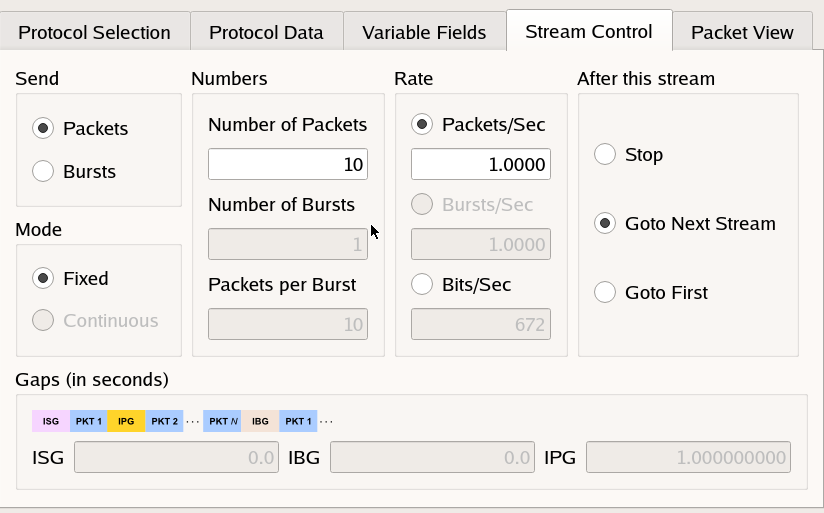
\includegraphics{data/q2.1-stream-settings.png}
\caption{Stream Settings for Question 2}
\end{figure}

The number of requests according to the stream settings is 10, which is
precisely what we observe.

\hypertarget{q2.2}{%
\section{(Q2.2)}\label{q2.2}}

486, 488, 490, 492, 494, 496, 500, 502, 504 and 506 are the numbers
associated with the request packets generated by Ostinato.

487, 489, 491, 493, 495, 497, 501, 503, 505 and 507 are the numbers
associated with the reply packets sent by the DUT (Device Under Test).

\hypertarget{q2.3}{%
\section{(Q2.3)}\label{q2.3}}

\[
\begin{aligned}
&\frac{
\begin{aligned}
&(4618.638764 - 4617.638757)
+(4619.638761 - 4618.638764)
+(4620.638772 - 4619.638761)\\
+\ &(4621.638731 - 4620.638772)
+(4622.638714 - 4621.638731)
+(4623.638729 - 4622.638714)\\
+\ &(4624.638727 - 4623.638729)
+(4625.638735 - 4624.638727)
+(4626.638725 - 4625.638735)
\end{aligned}
}{10 - 1}\\
=\ & 0.9999964444444535\ \text{seconds}
\end{aligned}
\]

The above computed value is the average interpacket gap i.e.~the delay
between request packets in seconds. It is approximately 1 second which
is precisely what was set in the stream settings. As is clearly visible
in the above picture.

Below is the Python 3 expression used to calculate the above value.

\begin{Shaded}
\begin{Highlighting}[]
\NormalTok{((}\FloatTok{4618.638764} \OperatorTok{{-}} \FloatTok{4617.638757}\NormalTok{)}
\OperatorTok{+}\NormalTok{(}\FloatTok{4619.638761} \OperatorTok{{-}} \FloatTok{4618.638764}\NormalTok{)}
\OperatorTok{+}\NormalTok{(}\FloatTok{4620.638772} \OperatorTok{{-}} \FloatTok{4619.638761}\NormalTok{)}
\OperatorTok{+}\NormalTok{(}\FloatTok{4621.638731} \OperatorTok{{-}} \FloatTok{4620.638772}\NormalTok{)}
\OperatorTok{+}\NormalTok{(}\FloatTok{4622.638714} \OperatorTok{{-}} \FloatTok{4621.638731}\NormalTok{)}
\OperatorTok{+}\NormalTok{(}\FloatTok{4623.638729} \OperatorTok{{-}} \FloatTok{4622.638714}\NormalTok{)}
\OperatorTok{+}\NormalTok{(}\FloatTok{4624.638727} \OperatorTok{{-}} \FloatTok{4623.638729}\NormalTok{)}
\OperatorTok{+}\NormalTok{(}\FloatTok{4625.638735} \OperatorTok{{-}} \FloatTok{4624.638727}\NormalTok{)}
\OperatorTok{+}\NormalTok{(}\FloatTok{4626.638725} \OperatorTok{{-}} \FloatTok{4625.638735}\NormalTok{))}\OperatorTok{/}\DecValTok{9}
\end{Highlighting}
\end{Shaded}

\hypertarget{q3}{%
\section{(Q3)}\label{q3}}

Below is picture of the updated settings.

\begin{figure}
\centering
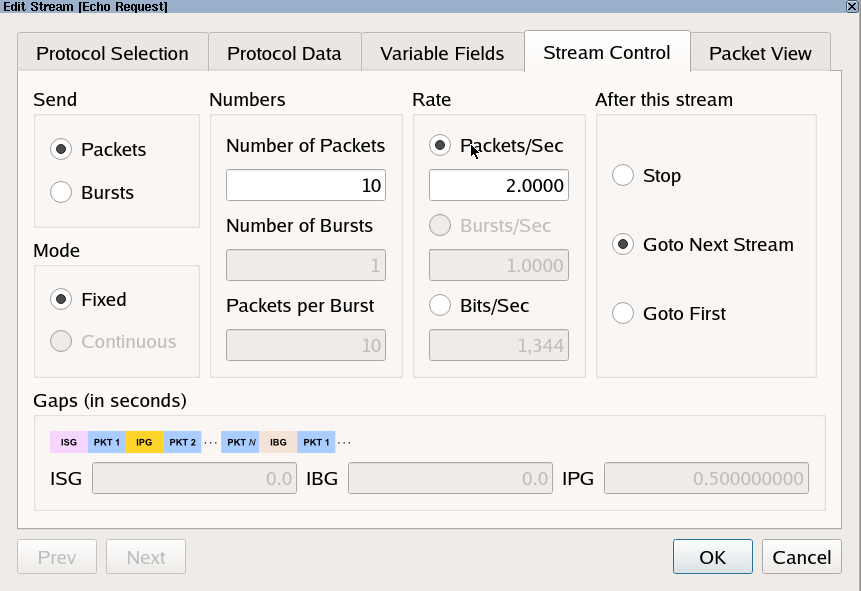
\includegraphics{data/q3-stream-settings.png}
\caption{Stream Settings for Question 3}
\end{figure}

And below here you can find the new capture.

\begin{longtable}[]{@{}
  >{\raggedright\arraybackslash}p{(\columnwidth - 12\tabcolsep) * \real{0.0263}}
  >{\raggedright\arraybackslash}p{(\columnwidth - 12\tabcolsep) * \real{0.0877}}
  >{\raggedright\arraybackslash}p{(\columnwidth - 12\tabcolsep) * \real{0.1053}}
  >{\raggedright\arraybackslash}p{(\columnwidth - 12\tabcolsep) * \real{0.1053}}
  >{\raggedright\arraybackslash}p{(\columnwidth - 12\tabcolsep) * \real{0.0702}}
  >{\raggedright\arraybackslash}p{(\columnwidth - 12\tabcolsep) * \real{0.0526}}
  >{\raggedright\arraybackslash}p{(\columnwidth - 12\tabcolsep) * \real{0.5526}}@{}}
\toprule
\begin{minipage}[b]{\linewidth}\raggedright
No.
\end{minipage} & \begin{minipage}[b]{\linewidth}\raggedright
Time
\end{minipage} & \begin{minipage}[b]{\linewidth}\raggedright
Source
\end{minipage} & \begin{minipage}[b]{\linewidth}\raggedright
Destination
\end{minipage} & \begin{minipage}[b]{\linewidth}\raggedright
Protocol
\end{minipage} & \begin{minipage}[b]{\linewidth}\raggedright
Length
\end{minipage} & \begin{minipage}[b]{\linewidth}\raggedright
Info
\end{minipage} \\
\midrule
\endhead
16 & 140.926179 & 192.168.0.10 & 192.168.0.1 & ICMP & 60 & Echo (ping)
request id=0x04d2, seq=0/0, ttl=127 (reply in 17) \\
17 & 140.926306 & 192.168.0.1 & 192.168.0.10 & ICMP & 60 & Echo (ping)
reply id=0x04d2, seq=0/0, ttl=64 (request in 16) \\
18 & 141.426171 & 192.168.0.10 & 192.168.0.1 & ICMP & 60 & Echo (ping)
request id=0x04d2, seq=0/0, ttl=127 (reply in 19) \\
19 & 141.426320 & 192.168.0.1 & 192.168.0.10 & ICMP & 60 & Echo (ping)
reply id=0x04d2, seq=0/0, ttl=64 (request in 18) \\
20 & 141.926165 & 192.168.0.10 & 192.168.0.1 & ICMP & 60 & Echo (ping)
request id=0x04d2, seq=0/0, ttl=127 (reply in 21) \\
21 & 141.926287 & 192.168.0.1 & 192.168.0.10 & ICMP & 60 & Echo (ping)
reply id=0x04d2, seq=0/0, ttl=64 (request in 20) \\
22 & 142.426145 & 192.168.0.10 & 192.168.0.1 & ICMP & 60 & Echo (ping)
request id=0x04d2, seq=0/0, ttl=127 (reply in 23) \\
23 & 142.426254 & 192.168.0.1 & 192.168.0.10 & ICMP & 60 & Echo (ping)
reply id=0x04d2, seq=0/0, ttl=64 (request in 22) \\
24 & 142.926106 & 192.168.0.10 & 192.168.0.1 & ICMP & 60 & Echo (ping)
request id=0x04d2, seq=0/0, ttl=127 (reply in 25) \\
25 & 142.926275 & 192.168.0.1 & 192.168.0.10 & ICMP & 60 & Echo (ping)
reply id=0x04d2, seq=0/0, ttl=64 (request in 24) \\
26 & 143.426150 & 192.168.0.10 & 192.168.0.1 & ICMP & 60 & Echo (ping)
request id=0x04d2, seq=0/0, ttl=127 (reply in 27) \\
27 & 143.426249 & 192.168.0.1 & 192.168.0.10 & ICMP & 60 & Echo (ping)
reply id=0x04d2, seq=0/0, ttl=64 (request in 26) \\
28 & 143.926104 & 192.168.0.10 & 192.168.0.1 & ICMP & 60 & Echo (ping)
request id=0x04d2, seq=0/0, ttl=127 (reply in 29) \\
29 & 143.926259 & 192.168.0.1 & 192.168.0.10 & ICMP & 60 & Echo (ping)
reply id=0x04d2, seq=0/0, ttl=64 (request in 28) \\
30 & 144.426138 & 192.168.0.10 & 192.168.0.1 & ICMP & 60 & Echo (ping)
request id=0x04d2, seq=0/0, ttl=127 (reply in 31) \\
31 & 144.426250 & 192.168.0.1 & 192.168.0.10 & ICMP & 60 & Echo (ping)
reply id=0x04d2, seq=0/0, ttl=64 (request in 30) \\
32 & 144.926075 & 192.168.0.10 & 192.168.0.1 & ICMP & 60 & Echo (ping)
request id=0x04d2, seq=0/0, ttl=127 (reply in 33) \\
33 & 144.926259 & 192.168.0.1 & 192.168.0.10 & ICMP & 60 & Echo (ping)
reply id=0x04d2, seq=0/0, ttl=64 (request in 32) \\
34 & 145.426128 & 192.168.0.10 & 192.168.0.1 & ICMP & 60 & Echo (ping)
request id=0x04d2, seq=0/0, ttl=127 (reply in 35) \\
35 & 145.426236 & 192.168.0.1 & 192.168.0.10 & ICMP & 60 & Echo (ping)
reply id=0x04d2, seq=0/0, ttl=64 (request in 34) \\
\bottomrule
\end{longtable}

Again the number of packets in total is 20. 10 requests and 10 replies
as specified in the stream.

The request packets are precisely numbers: 16, 18, 20, 22, 24, 26, 28,
30, 32, 34.

The reply packets are precisely numbers: 17, 19, 21, 23, 25, 27, 29, 31,
33, 35.

The average interpacket gap is roughly 0.5 seconds as calculated below.
This is also as expected as we increased the number of packets per
second from 1 to 2.

\[
\begin{aligned}
&\frac{
\begin{aligned}
&(141.426171 - 140.926179)
+(141.926165 - 141.426171)
+(142.426145 - 141.926165)\\
+\ &(142.926106 - 142.426145)
+(143.426150 - 142.926106)
+(143.926104 - 143.426150)\\
+\ &(144.426138 - 143.926104)
+(144.926075 - 144.426138)
+(145.426128 - 144.926075)
\end{aligned}
}{10 - 1}\\
=\ & 0.499994333333335\ \text{seconds}
\end{aligned}
\]

Below is the Python 3 expression used to calculate the above value.

\begin{Shaded}
\begin{Highlighting}[]
\NormalTok{((}\FloatTok{141.426171} \OperatorTok{{-}} \FloatTok{140.926179}\NormalTok{)}
\OperatorTok{+}\NormalTok{(}\FloatTok{141.926165} \OperatorTok{{-}} \FloatTok{141.426171}\NormalTok{)}
\OperatorTok{+}\NormalTok{(}\FloatTok{142.426145} \OperatorTok{{-}} \FloatTok{141.926165}\NormalTok{)}
\OperatorTok{+}\NormalTok{(}\FloatTok{142.926106} \OperatorTok{{-}} \FloatTok{142.426145}\NormalTok{)}
\OperatorTok{+}\NormalTok{(}\FloatTok{143.426150} \OperatorTok{{-}} \FloatTok{142.926106}\NormalTok{)}
\OperatorTok{+}\NormalTok{(}\FloatTok{143.926104} \OperatorTok{{-}} \FloatTok{143.426150}\NormalTok{)}
\OperatorTok{+}\NormalTok{(}\FloatTok{144.426138} \OperatorTok{{-}} \FloatTok{143.926104}\NormalTok{)}
\OperatorTok{+}\NormalTok{(}\FloatTok{144.926075} \OperatorTok{{-}} \FloatTok{144.426138}\NormalTok{)}
\OperatorTok{+}\NormalTok{(}\FloatTok{145.426128} \OperatorTok{{-}} \FloatTok{144.926075}\NormalTok{))}\OperatorTok{/}\DecValTok{9}
\end{Highlighting}
\end{Shaded}

\hypertarget{q4.1}{%
\section{(Q4.1)}\label{q4.1}}

The two packets under consideration are the ones below.

\begin{figure}
\centering
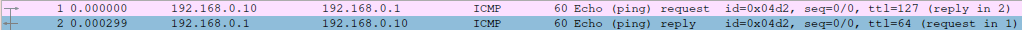
\includegraphics{data/q4.1-packets-under-inspection.png}
\caption{Packets Under Inspection for Question 4.1}
\end{figure}

The info related to the to the request from the generator to the DUT is
provided below. Specifically, the information related to the Ethernet II
frame.

\begin{figure}
\centering
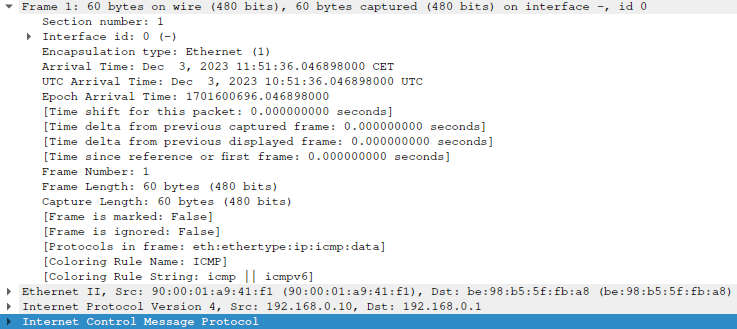
\includegraphics{data/q4.1-request-info.png}
\caption{Reply Info for Question 4.1}
\end{figure}

The number of bytes capture by Wireshark is exactly \(60\) bytes.

\hypertarget{q4.2}{%
\section{(Q4.2)}\label{q4.2}}

\begin{figure}
\centering
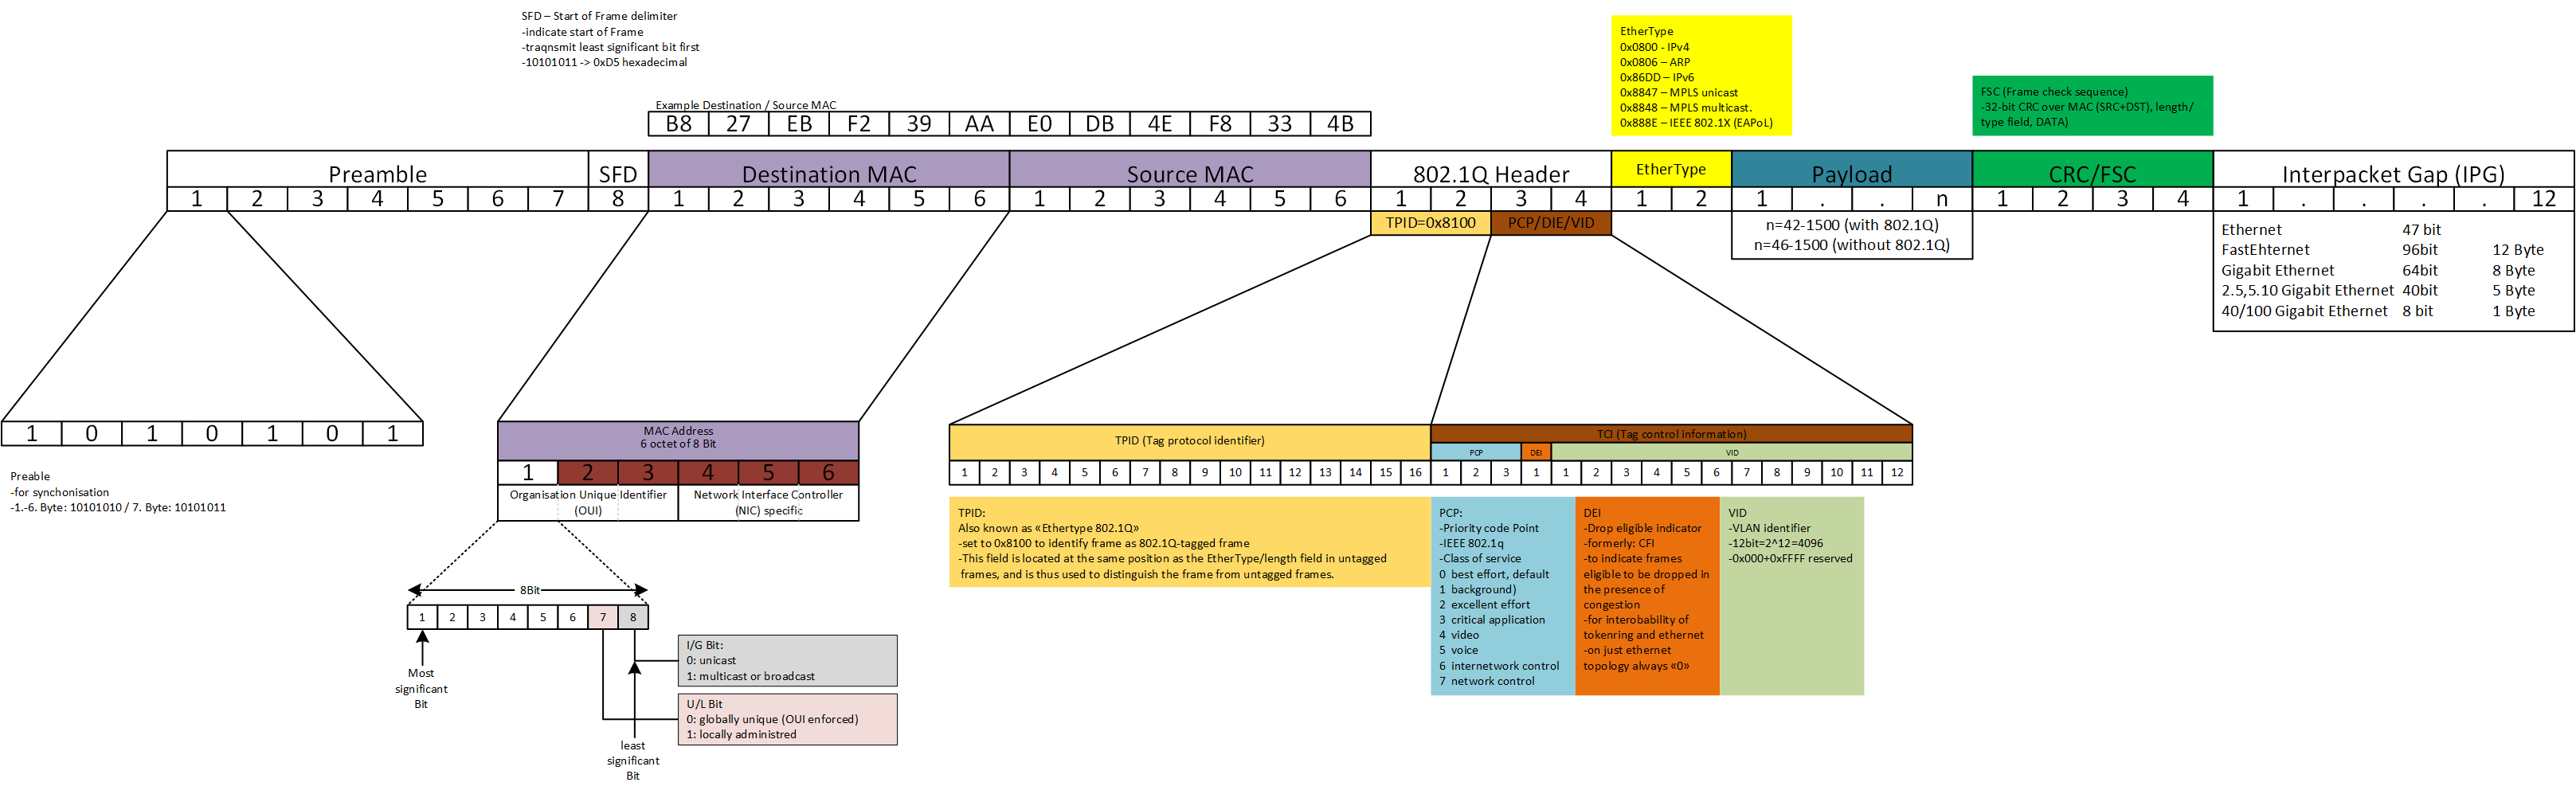
\includegraphics{data/q4.2-ethernet-diagram.png}
\caption{Ethernet II Frame for Question 4.2}
\end{figure}

\begin{quote}
\emph{Reference}:
https://upload.wikimedia.org/wikipedia/commons/7/72/Ethernet\_Frame.png

\textbf{Note}: There is a mistake in the graphic. ``CRC/FSC'' should be
``CRC/FCS'' and ``FSC (Frame check sequence)'' should be ``FCS (Frame
check sequence)''.
\end{quote}

The minimum and maximum lengths can be derived from the above image
using the fact that the Ethernet Frame at Layer 2 is comprised of the
following segments:

\begin{itemize}
\tightlist
\item
  Destination MAC (\(6\) octets);
\item
  Source MAC (\(6\) octets);
\item
  802.1Q Header (optional \& \(4\) octets);
\item
  EtherType (\(2\) octets);
\item
  Payload (\(42\) - \(1500\) octets with 802.1Q \& \(46\) - \(1500\)
  octets without 802.1Q); and
\item
  CRC/FCS (\(4\) octets).
\end{itemize}

Hence we can perform the following calculation for the minimum length:

\[
{\text{Frame}}_{\text{min}} = 6 + 6 + 2 + 46 + 4 = 64\ \text{octets}
\]

\begin{quote}
\textbf{Note}: In the case when we do not have a 802.1Q Header we get
\(0 + 46 = 46\) octets combined since the header has \(0\) length and
the Payload has a minimum length of \(46\). In the other case i.e.~when
we have a 802.1Q Header we get \(4 + 42 = 46\) octets which is exactly
the same as when we do not have a 802.1Q Header. Hence, both cases are
identical.
\end{quote}

Similarly, the maximum length is given by the following calculation:

\[
{\text{Frame}}_{\text{max}} = 6 + 6 + 2 + 1500 + 4 = 1518\ \text{octets}
\]

\hypertarget{q4.3}{%
\section{(Q4.3)}\label{q4.3}}

The number of ``bytes the wire'' according to Wireshark is precisely
\(60\) bytes. However, the minimum number of bytes is at least \(64\).
Hence, we have \(4\) bytes which are missing.

Now notice that the Ethernet Header does not contain an 802.1Q Header.
Hence we are allowed \(46\) bytes of Payload. These are all used up by
our ICMP Request (including all IP overhead).

\begin{figure}
\centering
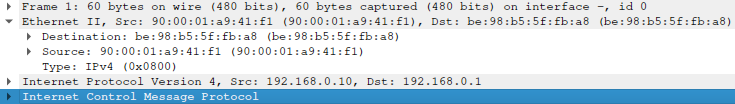
\includegraphics{data/q4.3-ethernet-header.png}
\caption{Ethernet Header for Question 4.3}
\end{figure}

Hence the Ethernet Header and ICMP Request total \(60\) bytes. This
means that our missing field is the Cyclic Redundancy Check (CRC) or
Frame Check Sequence (FCS). This field is precisely \(4\) bytes and
describes our discrepancy.

This is further supported by the following Wireshark forum discussion
which exclaims that ``bytes on wire'' is actually ``bytes on wire
without CRC''.

\begin{quote}
\emph{Reference}:
https://osqa-ask.wireshark.org/questions/1344/does-frame-length-include-also-crc-bytes
\end{quote}

\hypertarget{q4.4}{%
\section{(Q4.4)}\label{q4.4}}

Here are the source and destination addresses of the request as observed
above.

Source MAC = \texttt{90:00:01:a9:41:f1}

Destination MAC = \texttt{be:98:b5:5f:fb:a8}

\hypertarget{q4.5}{%
\section{(Q4.5)}\label{q4.5}}

\begin{figure}
\centering
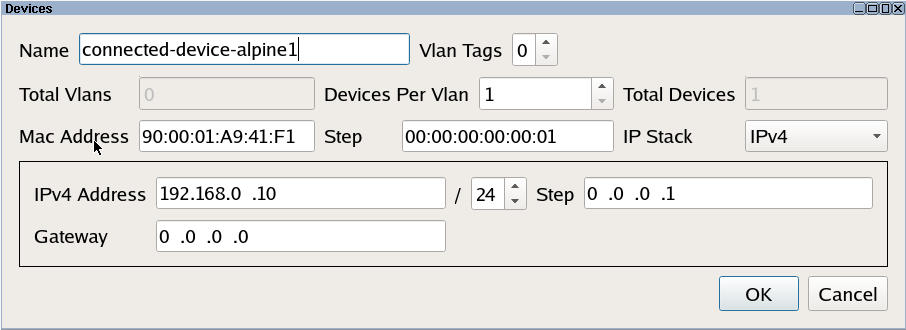
\includegraphics{data/q4.5-device-group-config.png}
\caption{Device Group Config for Question 4.5}
\end{figure}

\begin{quote}
\textbf{Note}: Since the device group contains as single device the base
MAC address i.e.~\texttt{90:00:01:a9:41:f1} is used for that device.
\end{quote}

The MAC address of our virtual device is \texttt{90:00:01:a9:41:f1}.

\hypertarget{q4.6}{%
\section{(Q4.6)}\label{q4.6}}

\begin{quote}
\textbf{Note}: Assuming that in the question, 5.4 and 5.5 where meant to
be 4.4 and 4.5 respectively.
\end{quote}

As we expected, the MAC Address of the virtual device is identical to
the Source MAC Address in the packet. This is because of the fact that
the packet is a Request packet i.e.~it was create by Ostinato.

It is also critical to point out that the request is very much dependant
on ARP (Address Resolution Protocol) requests to establish who has the
which is MAC addresses.

\hypertarget{q4.7}{%
\section{(Q4.7)}\label{q4.7}}

In previous sections I have reference the EtherType or Type field. I
also included a picture of the Ethernet Header of the Request packet.

The Type field is set to \texttt{0x0800} which refers to IPv4. Hence,
the receiver will understand that the Payload is an IPv4 packet and it
will be able to decode it.

\hypertarget{q4.8}{%
\section{(Q4.8)}\label{q4.8}}

\begin{figure}
\centering
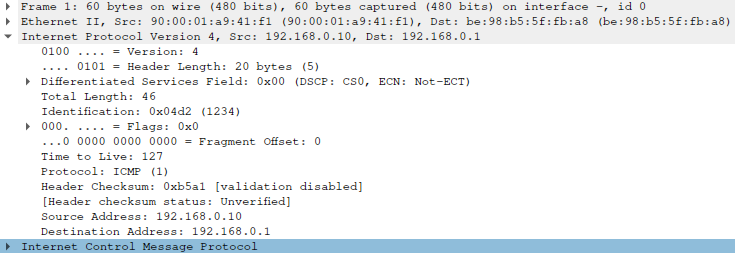
\includegraphics{data/q4.8-ip-header.png}
\caption{IP Header for Question 4.8}
\end{figure}

Source IP Address = \texttt{192.168.0.10}

Destination IP Address = \texttt{192.168.0.1}

These are precisely, the values we defined in the stream as can be seen
below.

\begin{figure}
\centering
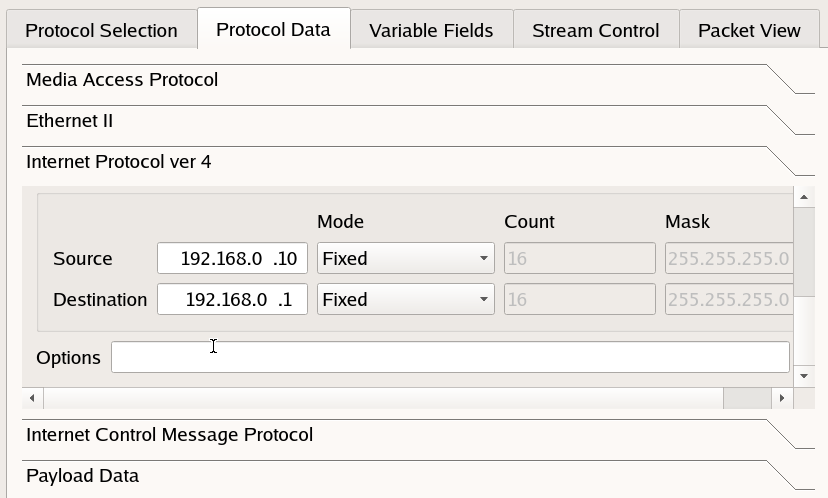
\includegraphics{data/q4.8-stream-config.png}
\caption{Stream IPv4 Config for Question 4.8}
\end{figure}

Additionally, the Total Length is \(46\) bytes. This is precisely what
we described before hand. The Ethernet Header Length is \(14\) bytes,
and \(14 + 46 = 60\) bytes as expected.

We can also be a bit more specific and point out that \(20\) of the
\(46\) bytes are the IPv4 Header Length whilst the remaining \(26\)
bytes are the actual ICMP Request.

\hypertarget{q5}{%
\section{(Q5)}\label{q5}}

\begin{figure}
\centering
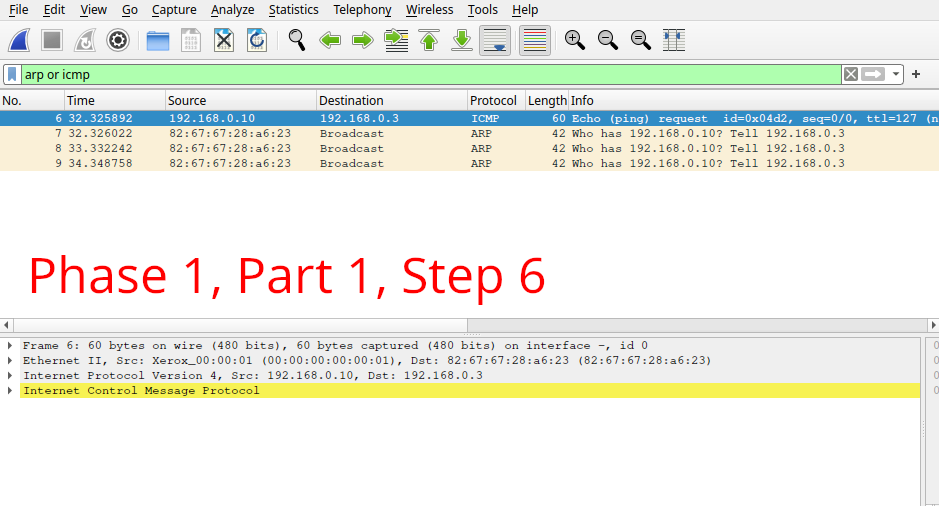
\includegraphics{data/q5-capture1.png}
\caption{Capture 1 for Question 5}
\end{figure}

\begin{figure}
\centering
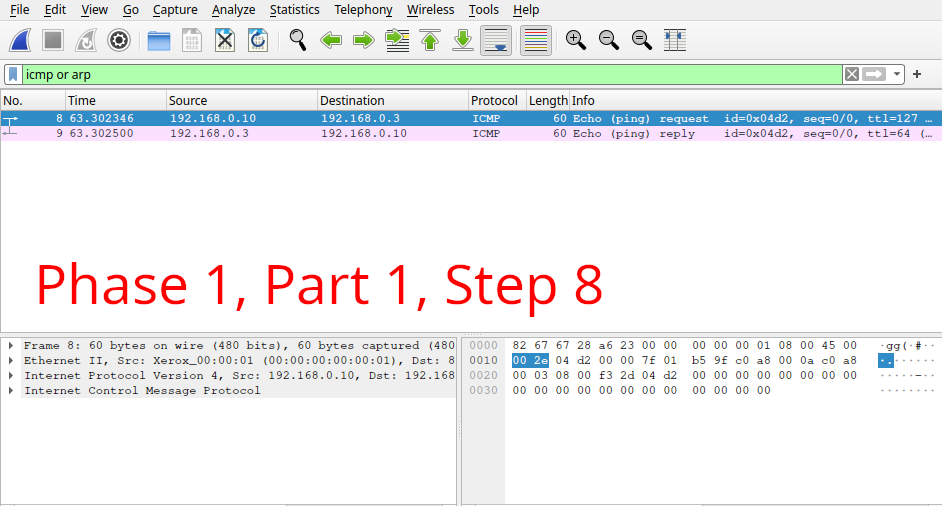
\includegraphics{data/q5-capture2.png}
\caption{Capture 2 for Question 5}
\end{figure}

\begin{figure}
\centering
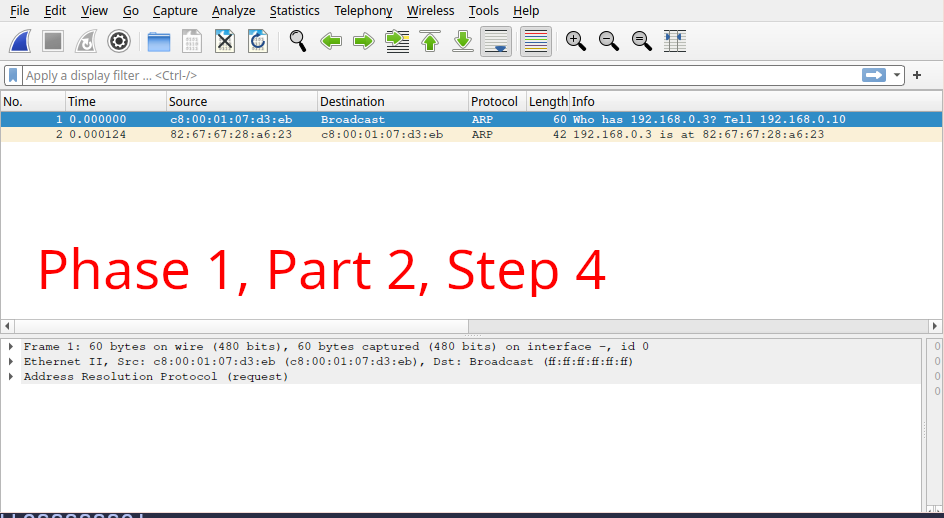
\includegraphics{data/q5-capture3.png}
\caption{Capture 3 for Question 5}
\end{figure}

\begin{figure}
\centering
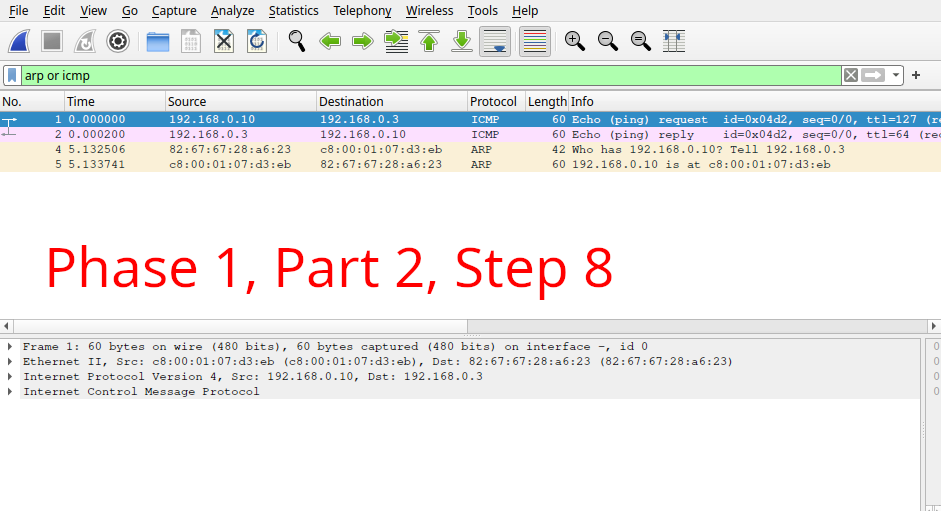
\includegraphics{data/q5-capture4.png}
\caption{Capture 4 for Question 5}
\end{figure}

The above four pictures are all the Wireshark captures as specified in
the lab sheet.

All we have to do is notice that the addresses in use are
\texttt{192.168.0.10} and \texttt{192.168.0.3}. The important thing to
note is that these are the IP addresses of the virtual Ostinato device
and the Alpine-3 Docker Container.

And we are doing so even though all these captures happened on the wire
between Hub1 and Apline-1. This essentially, exposes the nature of the
Hub as a networking device. Specifically, the Hub acts as a broadcasting
relay. It does not send packets only where they are required, it takes a
broad stroke approach and replays the packet it receives to every other
connection to the Hub.

\hypertarget{q6}{%
\section{(Q6)}\label{q6}}

So, for this question we will repeat all the steps described in Phase 1,
Part 2. However, this time we will use Port 1 or eth2() (in Ostinato)
and monitor both connections i.e.~Switch1 to apline-2 and Swtich1 to
apline-4.

This is because this will allows us to understand the nature of Switch
compared to a Hub.

\begin{figure}
\centering
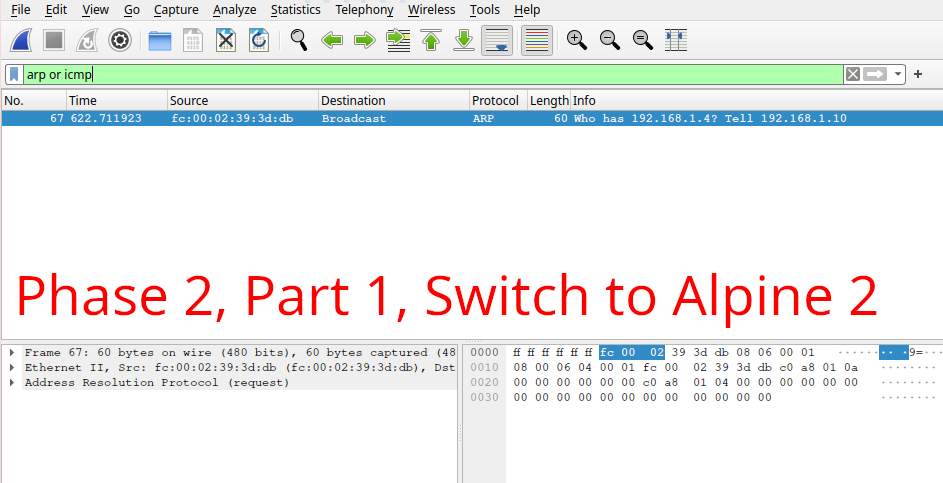
\includegraphics{data/q6-phase2-switch-to-alpine2-part1.png}
\caption{Switch to Apline 2 Part 1 for Question 6}
\end{figure}

\begin{figure}
\centering
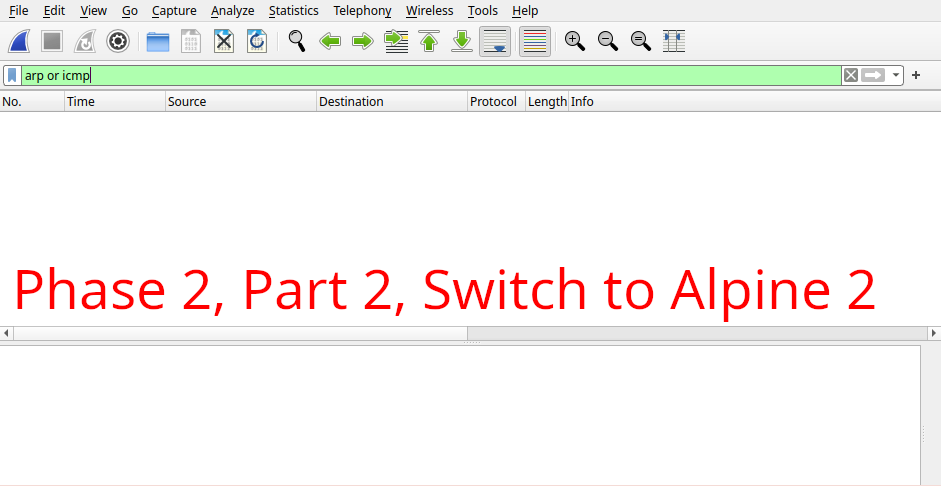
\includegraphics{data/q6-phase2-switch-to-alpine2-part2.png}
\caption{Switch to Apline 2 Part 2 for Question 6}
\end{figure}

Firstly, it is important to note that we only actually capture a single
packet on the Switch \textless-\textgreater{} Apline 2 connection as
clearly established by the pictures above, specifically Switch to Apline
2 Part 1 and Swithc to Apline 2 Part 2.

Additionally, the only difference between my output and that present in
Fig. 37 of the lab sheet is the MAC address. However, this could have
also been made the same since the MAC address can be set by the user of
Ostinato.

\hypertarget{q7.1}{%
\section{(Q7.1)}\label{q7.1}}

\begin{figure}
\centering
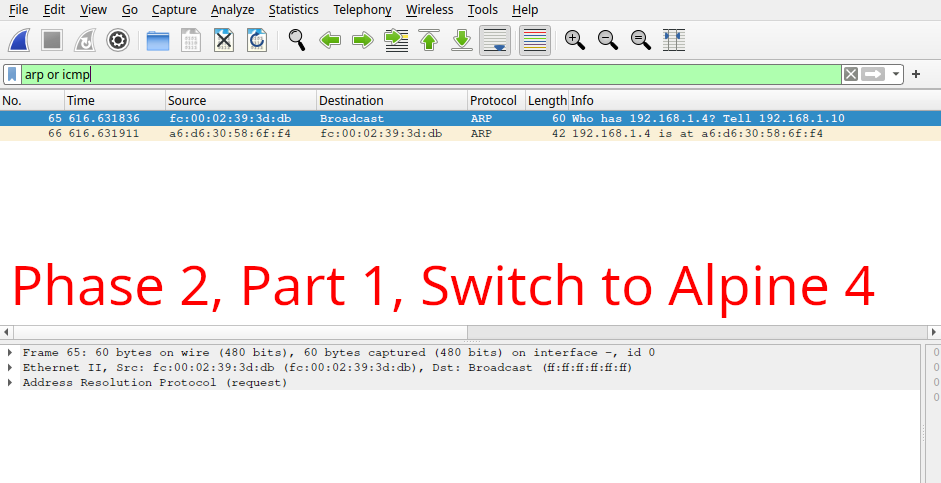
\includegraphics{data/q6-phase2-switch-to-alpine4-part1.png}
\caption{Switch to Apline 4 Part 1 for Question 6}
\end{figure}

\begin{figure}
\centering
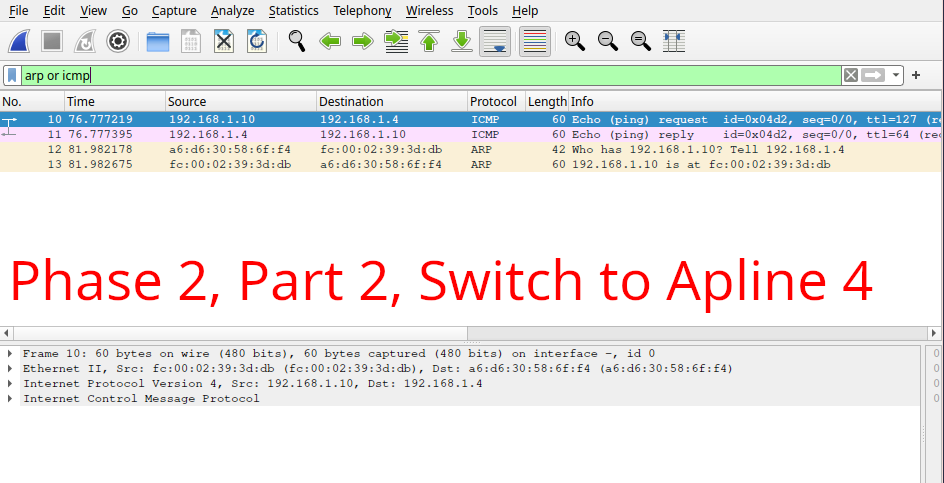
\includegraphics{data/q6-phase2-switch-to-alpine4-part2.png}
\caption{Switch to Apline 4 Part 2 for Question 6}
\end{figure}

\begin{quote}
\textbf{Note}: There are two screenshots is because I split the capture
into two separate captures.
\end{quote}

The above two screenshots show the packets captured over the Switch
\textless-\textgreater{} Alpine 4 connection.

\hypertarget{q7.2}{%
\section{(Q7.2)}\label{q7.2}}

So, from here onwards I will refer to the packets with there No. as
marked in the previous two screenshots. Specifically, these are 65, 66
\& 10, 11, 12, 13.

\begin{itemize}
\item
  Now 12 and 13 form part of the ARP request which apline-4 autonomously
  inserts as described in the lab sheet. Specifically, 12 is the request
  and 13 is the reply.
\item
  65 and 66 are the initial packets sent and these constitute the
  initial stage when we apply our configuration from within Ostinato.
  These packets form part of an ARP correspondence. ARP is used to
  establish whether or not the entity associated with the specified IP
  address is also an L2 entity in our local network. Additionally, if
  the entity is an L2 entity it replies back with its MAC address. This
  procedure happens via an initial request for discovery. In our case
  this request is 65. The device initiating ARP will broadcast an ARP
  request requesting the MAC Address of the current holder of the
  specified IP. Each device on the local network will receive this ARP
  request and then they will proceed to check whether or not they have
  the requested IP address. If they do they will send there MAC address
  as a unicast ARP request since the MAC address of the initiator is
  known since it would be the source MAC address in the initial
  broadcast. What I am describing is essentially, packet No.~66.
\item
  Finally, we shall discuss the actual interesting packets, specifically
  10 and 11. The ICMP request 10, is sent when we execute the stream we
  created in Ostinato. ICMPs are meant to check whether a device with
  the specified IP exists and whether it can service our request. This
  is the case for us and we get back a reply to our request. As can be
  seen the request is No.~11.
\end{itemize}

\hypertarget{q7.3}{%
\section{(Q7.3)}\label{q7.3}}
